\documentclass[conference]{IEEEtran}
\usepackage{cite}
\usepackage{amsmath,amssymb,amsfonts}
\usepackage{algorithm}
\usepackage{algorithmic}
\usepackage{graphicx}
\usepackage{textcomp}
\usepackage{xcolor}
\usepackage{booktabs}
\usepackage[utf8]{inputenc}
\usepackage[vietnamese]{babel}

\begin{document}

\title{Greedy Selection of Independent Labels for Multi-Label Classification with Partial Abstention}

\author{\IEEEauthorblockN{Anonymous Authors}
\IEEEauthorblockA{\textit{Department of Computer Science and Engineering} \\
\textit{Machine Learning Research Laboratory}\\
Email: author@university.edu.vn}
}

\maketitle

\begin{abstract}
Bài toán Multi-Label Classification (MLC) trong các miền ứng dụng quan trọng và có tính rủi ro cao (safety-critical) đòi hỏi mô hình phải cân bằng giữa predictive accuracy, tính khả thi về mặt tính toán và decision reliability. Classifier Chains (CC) mô hình hóa label dependencies bằng cách áp đặt một sequential directed acyclic graph (DAG) trên toàn bộ labels; tuy nhiên, CC chịu ảnh hưởng nặng nề bởi error propagation, computational complexity cao, và exact Bayes-optimal inference (BOP) là bài toán NP-hard. Hơn nữa, các mô hình MLC truyền thống luôn áp đặt mandatory predictions trên cả các labels có độ không chắc chắn cao, dẫn đến các sai số nghiêm trọng. Để giải quyết các thách thức này, bài báo đề xuất phương pháp Greedy Selection of Independent Labels for Multi-Label Classification with Partial Abstention (GSI-MLC-PA). Khung kiến trúc của chúng tôi phân hoạch thích nghi label space thành Independent Labels (IL) và Dependent Labels (DL) thông qua quy trình greedy selection trên internal validation split không rò rỉ dữ liệu. Các independent labels được ước lượng qua marginal estimators trực tiếp, trong khi dependent labels được mô hình hóa qua conditional chains kết hợp exact two-state marginalization và factorized mean-field plug-in approximation. Tầng quyết định Bayes-optimal tích hợp cho phép mô hình thực hiện partial abstention bằng cách trì hoãn dự đoán trên các vị trí label không chắc chắn dưới linear và concave penalties. Thực nghiệm toàn diện trên 10 benchmark datasets và 12 matched baseline architectures chứng minh GSI-MLC-PA đạt complete accuracy tương đương hoặc vượt trội (Hamming Accuracy đạt 0.9082 và Instance-F1 đạt 0.5659), đồng thời thu giữ hơn 90\% tổng số lỗi của hệ thống vào rejected label subset phục vụ quy trình human-in-the-loop review.
\end{abstract}

\begin{IEEEkeywords}
Multi-label classification, classifier chains, partial abstention, Bayes-optimal prediction, selective classification, label dependence.
\end{IEEEkeywords}

\section{Introduction}
Multi-label classification (MLC) là một bài toán nền tảng trong machine learning hiện đại, trong đó mỗi instance $x \in \mathcal{X}$ đồng thời được liên kết với một subset các labels từ label alphabet $\mathcal{L} = \{\lambda_1, \dots, \lambda_K\}$ \cite{zhang2018binary, read2011classifier}. Các ứng dụng thực tế từ clinical diagnosis, genomic annotation cho đến automated legal document tagging đều tồn tại pervasive semantic dependencies giữa các labels. Do đó, việc giả định các label variables hoàn toàn độc lập—tiêu biểu là mô hình Binary Relevance (BR) phân rã bậc một—thường thất bại trong việc nắm bắt joint label configurations và global subset constraints.

Để khai thác label interactions, Classifier Chains (CC) \cite{read2011classifier} và Probabilistic Classifier Chains (PCC) \cite{cheng2010bayes} chuyển đổi bài toán đa nhãn thành một quá trình sequential prediction dựa trên probability chain rule. Bằng cách sử dụng các dự đoán label phía trước làm augmented input features cho các classifiers phía sau, CC nắm bắt hiệu quả high-order correlations và cung cấp khả năng model interpretability (ví dụ: Shapley chain explanations) \cite{read2011classifier}. Mặc dù vậy, mô hình CC truyền thống bộc lộ ba điểm nghẽn nghiêm trọng:
\begin{enumerate}
    \item \textit{Error Propagation:} Sai số ở các mắt xích đầu tiên trong chain bị truyền trực tiếp sang downstream classifiers, kích hoạt hiện tượng cascading errors dọc theo chuỗi.
    \item \textit{Intractable Inference:} Việc xác định optimal chain permutation là bài toán NP-hard, và exact Bayes-Optimal Prediction (BOP) trên một fully connected chain đòi hỏi marginalizing trên exponential state space $2^K$.
    \item \textit{Mandatory Guessing under Uncertainty:} Trong các ứng dụng high-stakes, việc ép buộc đưa ra binary decisions khi marginal probabilities ở trạng thái phân vân ($p \approx 0.5$) làm suy giảm nghiêm trọng system trustworthiness.
\end{enumerate}

Để khắc phục các hạn chế cốt lõi trên, chúng tôi đề xuất mô hình \textbf{GSI-MLC-PA} (\textit{Greedy Selection of Independent labels for Multi-Label Classification with Partial Abstention}). GSI-MLC-PA phân tách label space thành hai tập: Independent Labels (IL) và Dependent Labels (DL) thông qua thuật toán greedy selection, cách ly rò rỉ trên internal validation data. Các independent labels được tách khỏi chuỗi tuần tự, triệt tiêu spurious error propagation. Các dependent labels được ước lượng thông qua exact two-state marginalization cho trường hợp single predecessor và continuous mean-field plug-in approximation cho multi-parent configurations, giảm inference complexity từ $\mathcal{O}(2^K)$ xuống polynomial time. Đồng thời, GSI-MLC-PA tích hợp tầng partial abstention dựa trên generalized Bayes-optimal decision theory \cite{nguyen2021multilabel}, cho phép xuất ra các quyết định $\{-1, 0, 1\}$ (với $-1$ đại diện cho abstention) nhằm chuyển giao các vị trí khó khăn cho human-in-the-loop review.

Các đóng góp chính của công trình bao gồm:
\begin{itemize}
    \item Đề xuất khung kiến trúc GSI-MLC-PA hoàn chỉnh, tích hợp adaptive IL/DL structural partitioning, exact và mean-field chain marginalization, cùng Bayes-optimal partial abstention thành một end-to-end learning pipeline.
    \item Xây dựng các thuật toán vectorized dynamic programming hiệu quả cho các Bayes-optimal decision policies dưới generalized Hamming loss, instance-based F-measure, và Jaccard utility, chứng minh việc phân rã cấu trúc IL/DL giúp tăng tốc inference và hạn chế error propagation.
    \item Thực nghiệm nghiêm ngặt và toàn diện trên 10 benchmark datasets với 600 outer cross-validation folds, 12 matched model configurations (gồm Logistic Regression, PyTorch MLPs tối ưu trên GPU, và Calibrated Support Vector Machines), chứng minh GSI-MLC-PA đạt risk-coverage trade-offs và error capture rates vượt trội.
\end{itemize}

Bố cục của bài báo: Section II tổng quan related work. Section III trình bày formal mathematical methodology và algorithmic logic. Section IV phân tích thực nghiệm và ablation studies. Section V tổng kết và nêu định hướng future work.

\section{Related Work}
\subsection{Label Correlation Modeling trong Multi-Label Learning}
Các thuật toán multi-label learning được phân loại thành first-order, second-order, và high-order approaches dựa trên cơ chế xử lý label dependencies \cite{zhang2018binary}. Binary Relevance (BR) là first-order baseline kinh điển, phân rã bài toán thành $K$ independent binary tasks. Mặc dù có $\mathcal{O}(K)$ complexity và tự nhiên kháng lại error propagation, BR bỏ qua label correlations, dẫn đến suboptimal subset accuracy và structured losses.

High-order methods mô hình hóa các mối quan hệ phức tạp giữa các label subsets tùy ý. Classifier Chains (CC) \cite{read2011classifier} xây dựng directed chain nơi mỗi classifier được huấn luyện trên original features kết hợp với preceding binary labels. Probabilistic Classifier Chains (PCC) \cite{cheng2010bayes} chuẩn hóa quy trình này qua conditional probability estimation $P(y|x) = \prod_{k=1}^K P(y_k|x, y_1, \dots, y_{k-1})$. Mặc dù PCC hỗ trợ Bayes-optimal inference về mặt lý thuyết, việc tìm kiếm maximizing label configuration trên $y \in \{0,1\}^K$ là bài toán NP-hard \cite{dembczynski2012consistent}. Các approximate search strategies như beam search, Monte Carlo sampling, và genetic algorithms \cite{read2012monte} chỉ giảm nhẹ chi phí tính toán nhưng vẫn dễ bị tổn thương khi predecessor predictions sai lệch.

\subsection{Selective Classification và Partial Abstention}
Selective classification (classification with a reject option) cho phép mô hình abstain khi uncertainty vượt quá predefined threshold \cite{geifman2017selective}. Trong multi-class settings, việc từ chối thường diễn ra ở instance-level. Tuy nhiên, trong multi-label learning, instance-level abstention là quá khắt khe, vì một instance có thể có certainty rất cao ở nhiều labels trong khi chỉ mơ hồ ở một vài labels cụ thể.

Nguyen và H\"ullermeier \cite{nguyen2021multilabel} đã hình thức hóa \textit{partial abstention} cho multi-label classification trong decision-theoretic framework. Không gian dự đoán được mở rộng thành $\{-1, 0, 1\}^K$, với $-1$ thể hiện abstention trên label thứ $k$. Hệ thống chịu generalized loss kết hợp misclassification penalties trên decided labels với một parametric penalty function $g(a)$ trên số lượng abstentions $a$. Họ đã thiết lập optimal rejection thresholds cho Hamming loss dưới linear penalty (SEP) và concave penalty (PAR), cùng dynamic programming formulations cho non-linear metrics như F-measure và Jaccard similarity. Tuy nhiên, framework của họ giả định marginal probabilities đã được calibrate hoàn hảo từ trước và chưa giải quyết structural complexity hay error cascades của classifier chains. GSI-MLC-PA kết nối trực tiếp khoảng trống này bằng cách kết hợp adaptive structural simplification với generalized decision-theoretic abstention.

\section{Methodology}

\subsection{Problem Formulation và Ký Hiệu Toán Học}
Gọi $\mathcal{X} \subseteq \mathbb{R}^d$ là $d$-dimensional input feature space và $\mathcal{Y} = \{0, 1\}^K$ là label space gồm $K$ binary labels $\mathcal{L} = \{\lambda_1, \dots, \lambda_K\}$. Training dataset $\mathcal{D} = \{(x_i, y_i)\}_{i=1}^N$ chứa $N$ i.i.d. instances từ joint distribution $\mathcal{P}(\mathcal{X}, \mathcal{Y})$, với $y_i = (y_{i,1}, \dots, y_{i,K})^\top \in \mathcal{Y}$.

Trong multi-label classification with partial abstention, prediction vector $\hat{y} \in \{-1, 0, 1\}^K$ cho phép ba actions trên mỗi label position $k \in \{1, \dots, K\}$:
\begin{equation}
    \hat{y}_k = \begin{cases}
        1, & \text{dự đoán label } \lambda_k \text{ xuất hiện}, \\
        0, & \text{dự đoán label } \lambda_k \text{ vắng mặt}, \\
        -1, & \text{abstain trên label } \lambda_k.
    \end{cases}
\end{equation}
Gọi $D(\hat{y}) = \{k \in \{1, \dots, K\} \mid \hat{y}_k \neq -1\}$ là tập các decided label indices, và $A(\hat{y}) = \{1, \dots, K\} \setminus D(\hat{y})$ là tập các abstained indices, với $a = |A(\hat{y})|$.

\subsection{Adaptive Label Partitioning (IL/DL)}
Để giải tỏa gánh nặng tính toán và triệt tiêu error propagation của full chains, GSI-MLC-PA phân rã $\mathcal{L}$ thành tập Independent Labels $\mathcal{I}$ và Dependent Labels $\mathcal{D}_L$, thỏa mãn $\mathcal{I} \cup \mathcal{D}_L = \mathcal{L}$ và $\mathcal{I} \cap \mathcal{D}_L = \emptyset$.

\subsubsection{Marginal Estimation cho Independent Labels}
Với mỗi label $\lambda_k \in \mathcal{I}$, marginal posterior probability được ước lượng từ input $x$ thông qua Binary Relevance estimator $h_k^{\text{BR}}: \mathcal{X} \to [0, 1]$:
\begin{equation}
    p_k^{\text{dir}}(x) = P(y_k = 1 \mid x) \approx h_k^{\text{BR}}(x).
\end{equation}

\subsubsection{Marginalization cho Dependent Labels}
Với label $\lambda_k \in \mathcal{D}_L$, dự đoán phụ thuộc vào preceding labels được định nghĩa bởi chain order $\pi = (\pi_1, \dots, \pi_K)$. Gọi $\text{Pred}(k) = \{\pi_j \mid j < \pi^{-1}(k)\}$ là tập predecessor labels của label $k$. Conditional classifier ước lượng:
\begin{equation}
    q_k(x, y_{\text{Pred}(k)}) = P(y_k = 1 \mid x, y_{\text{Pred}(k)}).
\end{equation}
Để thu được marginal probability $p_k(x) = P(y_k = 1 \mid x)$ mà không yêu cầu hard binary predecessor commitments, GSI-MLC-PA thực hiện marginalization:
\begin{itemize}
    \item \textbf{Exact Two-State Marginalization ($|\text{Pred}(k)| = 1$):} Khi $\text{Pred}(k) = \{m\}$, marginal probability được tính giải tích chính xác:
    \begin{equation}
        p_k(x) = (1 - p_m(x)) q_k(x, 0) + p_m(x) q_k(x, 1).
    \end{equation}
    \item \textbf{Factorized Mean-Field Plug-in ($|\text{Pred}(k)| \ge 2$):} Việc tính tổng trên $2^{|\text{Pred}(k)|}$ states là intractable. Dưới variational mean-field theory, joint posterior distribution của predecessor labels được xấp xỉ bằng factorized product $Q(y_{\text{Pred}(k)}) = \prod_{m \in \text{Pred}(k)} p_m(x)^{y_m} (1 - p_m(x))^{1 - y_m}$. Continuous expectations được đưa trực tiếp vào conditional estimator:
    \begin{equation}
        p_k(x) \approx q_k\left(x, \mathbf{p}_{\text{Pred}(k)}(x)\right),
    \end{equation}
    trong đó $\mathbf{p}_{\text{Pred}(k)}(x) = \left(p_m(x)\right)_{m \in \text{Pred}(k)} \in [0, 1]^{|\text{Pred}(k)|}$.
\end{itemize}

\subsection{Greedy Label Selection Algorithm}
Phân hoạch tối ưu $(\mathcal{I}, \mathcal{D}_L)$ được xác định thông qua greedy search trên internal validation split $\mathcal{D}_{\text{val}} \subset \mathcal{D}_{\text{train}}$, hoàn toàn không rò rỉ dữ liệu test bên ngoài.

Algorithm 1 mô tả chi tiết quy trình. Bắt đầu với toàn bộ labels khởi tạo trong $\mathcal{D}_L$ (tương đương standard CC), mỗi label lần lượt được chuyển sang $\mathcal{I}$. Candidate partition chỉ được chấp thuận nếu làm tăng ngặt internal validation objective $\mathcal{M}(\mathcal{D}_{\text{val}})$. Sau khi chốt partition, correlation matrix $\mathbf{R} \in [-1, 1]^{K \times K}$ được tính toán qua Pearson's $\phi$:
\begin{equation}
    \mathbf{R}_{j, k} = \frac{\sum_{i=1}^N (y_{i,j} - \bar{y}_j)(y_{i,k} - \bar{y}_k)}{\sqrt{\sum_{i=1}^N (y_{i,j} - \bar{y}_j)^2 \sum_{i=1}^N (y_{i,k} - \bar{y}_k)^2}}.
\end{equation}
Independent labels được lập lịch ở đầu chuỗi, và dependent labels được sắp xếp tuần tự bằng cách tối đa hóa absolute correlation với các nodes đã được lên lịch trước đó.

\begin{algorithm}[htbp]
\caption{Greedy Selection of Independent Labels (GSI)}
\begin{algorithmic}[1]
\REQUIRE Training set $\mathcal{D}_{\text{train}}$, validation fraction $\alpha \in (0, 1)$, objective $\mathcal{M}$.
\ENSURE Partition $(\mathcal{I}, \mathcal{D}_L)$, chain order $\pi$, refitted models $h^{\text{BR}}, h^{\text{CC}}$.
\STATE Split $\mathcal{D}_{\text{train}}$ into $\mathcal{D}_{\text{fit}}$ and $\mathcal{D}_{\text{val}}$ using stratified sampling.
\STATE Fit initial $h^{\text{BR}}$ and $h^{\text{CC}}$ on $\mathcal{D}_{\text{fit}}$.
\STATE Initialize $\mathcal{I} \leftarrow \emptyset$, $\mathcal{D}_L \leftarrow \{1, \dots, K\}$.
\STATE Compute baseline validation score: $S^* \leftarrow \mathcal{M}(h(\mathcal{D}_{\text{val}}; \mathcal{I}, \mathcal{D}_L))$.
\FOR{each label $k \in \{1, \dots, K\}$}
    \STATE Candidate partition: $\mathcal{I}' \leftarrow \mathcal{I} \cup \{k\}$, $\mathcal{D}_L' \leftarrow \mathcal{D}_L \setminus \{k\}$.
    \STATE Evaluate candidate score: $S' \leftarrow \mathcal{M}(h(\mathcal{D}_{\text{val}}; \mathcal{I}', \mathcal{D}_L'))$.
    \IF{$S' > S^*$}
        \STATE $\mathcal{I} \leftarrow \mathcal{I}'$, $\mathcal{D}_L \leftarrow \mathcal{D}_L'$, $S^* \leftarrow S'$.
    \ENDIF
\ENDFOR
\STATE Compute correlation matrix $\mathbf{R}$ from $\mathcal{D}_{\text{train}}$.
\STATE Construct correlation order $\pi$: schedule $\mathcal{I}$ first, then greedily append $m \in \mathcal{D}_L$ maximizing $\max_{j \in \text{scheduled}} |\mathbf{R}_{m, j}|$.
\STATE Refit $h^{\text{BR}}$ and $h^{\text{CC}}$ on full $\mathcal{D}_{\text{train}}$ using frozen partition $(\mathcal{I}, \mathcal{D}_L)$ and order $\pi$.
\RETURN $(\mathcal{I}, \mathcal{D}_L)$, $\pi$, $h^{\text{BR}}$, $h^{\text{CC}}$.
\end{algorithmic}
\end{algorithm}

\subsection{Bayes-Optimal Partial Abstention Layer}
Sau khi thu được marginal probabilities $\mathbf{p}(x) \in [0, 1]^K$, Bayes-optimal decision policy ánh xạ $\mathbf{p}(x)$ thành $\hat{y} \in \{-1, 0, 1\}^K$.

\subsubsection{Generalized Hamming Loss Formulation}
Dưới generalized Hamming loss, hàm mục tiêu được định nghĩa:
\begin{equation}
    \mathcal{L}_H(y, \hat{y}) = \sum_{k \in D(\hat{y})} \mathbb{I}(y_k \neq \hat{y}_k) + g(|A(\hat{y})|),
\end{equation}
với $g(a)$ là monotonic abstention penalty:
\begin{itemize}
    \item \textbf{Linear Penalty (SEP):} $g(a) = a \cdot c$, với cost parameter $c \in [0, 0.5]$. Do loss phân rã tuyến tính độc lập theo từng label position, Bayes-optimal decision rule là:
    \begin{equation}
        \hat{y}_k = \begin{cases}
            1, & \text{nếu } p_k(x) \ge 1 - c, \\
            0, & \text{nếu } p_k(x) \le c, \\
            -1, & \text{nếu } c < p_k(x) < 1 - c.
        \end{cases}
    \end{equation}
    \item \textbf{Concave Penalty (PAR):} $g(a) = \frac{a K c}{K + a}$, mô hình hóa diminishing returns của human inspection. Labels được sắp xếp tăng dần theo marginal decision risk $r_k = \min(p_k, 1 - p_k)$. Số lượng decisions tối ưu $d^* = |D(\hat{y})|$ được tìm trong thời gian $\mathcal{O}(K \log K)$:
    \begin{equation}
        d^* = \arg\min_{d \in \{0, \dots, K\}} \left\{ \sum_{j=1}^d r_{(j)} + g(K - d) \right\}.
    \end{equation}
\end{itemize}

\subsubsection{Dynamic Programming cho Instance F-Measure và Jaccard BOP}
Đối với non-decomposable metrics như Instance-F1 và Instance Jaccard, việc tối đa hóa expected utility dưới conditional label independence đòi hỏi đánh giá Poisson-binomial distribution convolutions. GSI-MLC-PA cài đặt các giải thuật vectorized $\mathcal{O}(K^3)$ dynamic programming (mở rộng Algorithm 2 và 3 của Nguyen-H\"ullermeier) bằng cách tiền tính toán prefix và suffix count distribution tables qua fast array operations, đảm bảo sub-second inference ngay cả trên datasets có hàng trăm labels.

\section{Experiments and Results}

\subsection{Experimental Setup}
\subsubsection{Benchmark Datasets}
Mô hình được đánh giá trên 10 benchmark multi-label datasets thuộc nhiều domains và dimensional scales: Emotions, Music, Scene, Yeast, Genbase, Medical, Enron, CAL500, Bibtex, và Reuters-K500. Table \ref{tab:datasets_vi} tóm tắt đặc trưng chính.

\begin{table}[htbp]
\caption{Benchmark Dataset Characteristics}
\label{tab:datasets_vi}
\centering
\begin{tabular}{lrrrrr}
\toprule
\textbf{Dataset} & \textbf{Domain} & \textbf{Instances} & \textbf{Features} & \textbf{Labels} & \textbf{Cardinality} \\
\midrule
Emotions & Music & 593 & 72 & 6 & 1.868 \\
Music & Music & 592 & 71 & 6 & 1.873 \\
Scene & Image & 2,407 & 294 & 6 & 1.074 \\
Yeast & Biology & 2,417 & 103 & 14 & 4.237 \\
Genbase & Biology & 662 & 1,186 & 27 & 1.252 \\
Medical & Text & 978 & 1,449 & 45 & 1.245 \\
Enron & Text & 1,702 & 1,001 & 53 & 3.378 \\
CAL500 & Music & 502 & 68 & 174 & 26.044 \\
Bibtex & Text & 7,395 & 1,836 & 159 & 2.402 \\
Reuters-K500 & Text & 6,000 & 500 & 103 & 1.462 \\
\bottomrule
\end{tabular}
\end{table}

\subsubsection{Matched Baseline Architectures}
Để loại bỏ confounding factors từ base-learner discrepancies, chúng tôi đánh giá một fully matched $4 \times 3$ model matrix:
\begin{itemize}
    \item \textbf{Model Families:} Binary Relevance (BR), Classifier Chains (CC), Multi-Label Classification with Partial Abstention (MLC-PA), và GSI-MLC-PA.
    \item \textbf{Base Learners:} (1) L2-regularized Logistic Regression (LIBLINEAR); (2) GPU-accelerated PyTorch Multi-Layer Perceptrons (MLP) với AdamW và BCEWithLogitsLoss; và (3) Linear Support Vector Machines calibrated qua nested out-of-fold Platt scaling (Calibrated LinearSVC).
\end{itemize}
Tất cả models được đánh giá qua 5-fold stratified cross-validation (tổng cộng 600 outer folds). Operating costs $c \in \{0.20, 0.25, 0.30, 0.35, 0.40, 0.50\}$ được chọn hoàn toàn trên inner validation folds.

\subsubsection{Evaluation Metrics}
Hiệu năng được đo lường trên bốn evaluation scopes:
\begin{enumerate}
    \item \textbf{Complete Metrics (Immediate Mode):} Hamming Accuracy ($1 - \text{Hamming Loss}$), Subset Accuracy, Macro-F1, Micro-F1, Instance-F1, và Instance Jaccard.
    \item \textbf{Selective Metrics:} Coverage ($\frac{|D(\hat{y})|}{N \cdot K}$), Selective Macro-F1, Selective Micro-F1, và Selective Hamming Accuracy.
    \item \textbf{Rejected Set Diagnostics:} Average Abstention per Sample (AABS), Abstention Rate (ABS), và Error Capture Rate ($\text{ECR} = \frac{\text{Errors in } A(\hat{y})}{\text{Total Full Errors}}$).
    \item \textbf{Optimistic Upper Bound:} Optimistic Macro-F1 giả định 100\% human reviewer precision trên các abstained positions.
\end{enumerate}

\subsection{Empirical Results và Comparative Analysis}

\subsubsection{Complete Prediction Performance (Zero Abstention)}
Table \ref{tab:complete_results_vi} báo cáo overall mean performance trên cả 10 benchmark datasets khi mô hình bắt buộc phải đưa ra immediate decisions ($c = 0.5$, không cho phép abstention).

\begin{table*}[htbp]
\caption{Overall Complete Prediction Performance Across 10 Benchmark Datasets (Mean over 50 Folds per Model)}
\label{tab:complete_results_vi}
\centering
\begin{tabular}{lcccccc}
\toprule
\textbf{Model Identifier} & \textbf{Hamming Acc. $\uparrow$} & \textbf{Macro-F1 $\uparrow$} & \textbf{Micro-F1 $\uparrow$} & \textbf{Instance-F1 $\uparrow$} & \textbf{Instance Jaccard $\uparrow$} & \textbf{Subset Acc. $\uparrow$} \\
\midrule
BR\_Logistic & 0.9079 & 0.3979 & 0.6105 & 0.5632 & 0.5010 & 0.3337 \\
BR\_MLP & 0.7731 & 0.3251 & 0.3710 & 0.3672 & 0.2676 & 0.0527 \\
BR\_SVM & 0.9059 & 0.3836 & 0.5870 & 0.5382 & 0.4782 & 0.3220 \\
\midrule
CC\_Logistic & 0.9008 & 0.4046 & 0.6111 & 0.5828 & 0.5237 & \textbf{0.3673} \\
CC\_MLP & 0.8569 & 0.3775 & 0.5558 & 0.5395 & 0.4516 & 0.2088 \\
CC\_SVM & 0.9001 & 0.4005 & 0.5990 & 0.5784 & 0.5188 & 0.3662 \\
\midrule
MLC\_PA\_Logistic & 0.9079 & 0.3979 & 0.6105 & 0.5632 & 0.5010 & 0.3337 \\
MLC\_PA\_MLP & 0.7731 & 0.3251 & 0.3710 & 0.3672 & 0.2676 & 0.0527 \\
MLC\_PA\_SVM & 0.9059 & 0.3836 & 0.5870 & 0.5382 & 0.4782 & 0.3220 \\
\midrule
GSI\_MLC\_PA\_Logistic & \textbf{0.9082} & 0.3986 & \textbf{0.6116} & 0.5659 & 0.5054 & 0.3431 \\
GSI\_MLC\_PA\_MLP & 0.8362 & 0.3377 & 0.4400 & 0.4133 & 0.3218 & 0.0933 \\
GSI\_MLC\_PA\_SVM & 0.9059 & \textbf{0.4009} & 0.5975 & 0.5554 & 0.4945 & 0.3358 \\
\bottomrule
\end{tabular}
\end{table*}

Kết quả thực nghiệm chứng minh:
\begin{enumerate}
    \item \textbf{Structural Simplification Bảo Toàn Accuracy:} GSI\_MLC\_PA\_Logistic đạt Hamming Accuracy cao nhất toàn cục (0.9082) và Micro-F1 cao nhất (0.6116), vượt qua cả BR\_Logistic (0.9079) lẫn standard CC\_Logistic (0.9008). Điều này khẳng định việc greedy pruning các uninformative chain predecessors chuyển sang independent set $\mathcal{I}$ ngăn chặn hiệu quả error propagation mà không đánh mất representative capacity.
    \item \textbf{Rigorous Baseline Invariance:} Table \ref{tab:complete_results_vi} xác nhận MLC\_PA và BR cho predictions hoàn toàn trùng khớp 100\% trên toàn bộ base learners, kiểm chứng tính đúng đắn của mathematical invariant khi Bayes-optimal thresholding suy biến về memoryless baseline tại cost $c = 0.5$.
    \item \textbf{Support Vector Machine Enhancement:} Dưới calibrated SVM backend, GSI\_MLC\_PA\_SVM đạt Macro-F1 0.4009, vượt trội đáng kể so với BR\_SVM (0.3836) và ngang hàng với CC\_SVM (0.4005).
\end{enumerate}

\begin{figure*}[htbp]
\centering
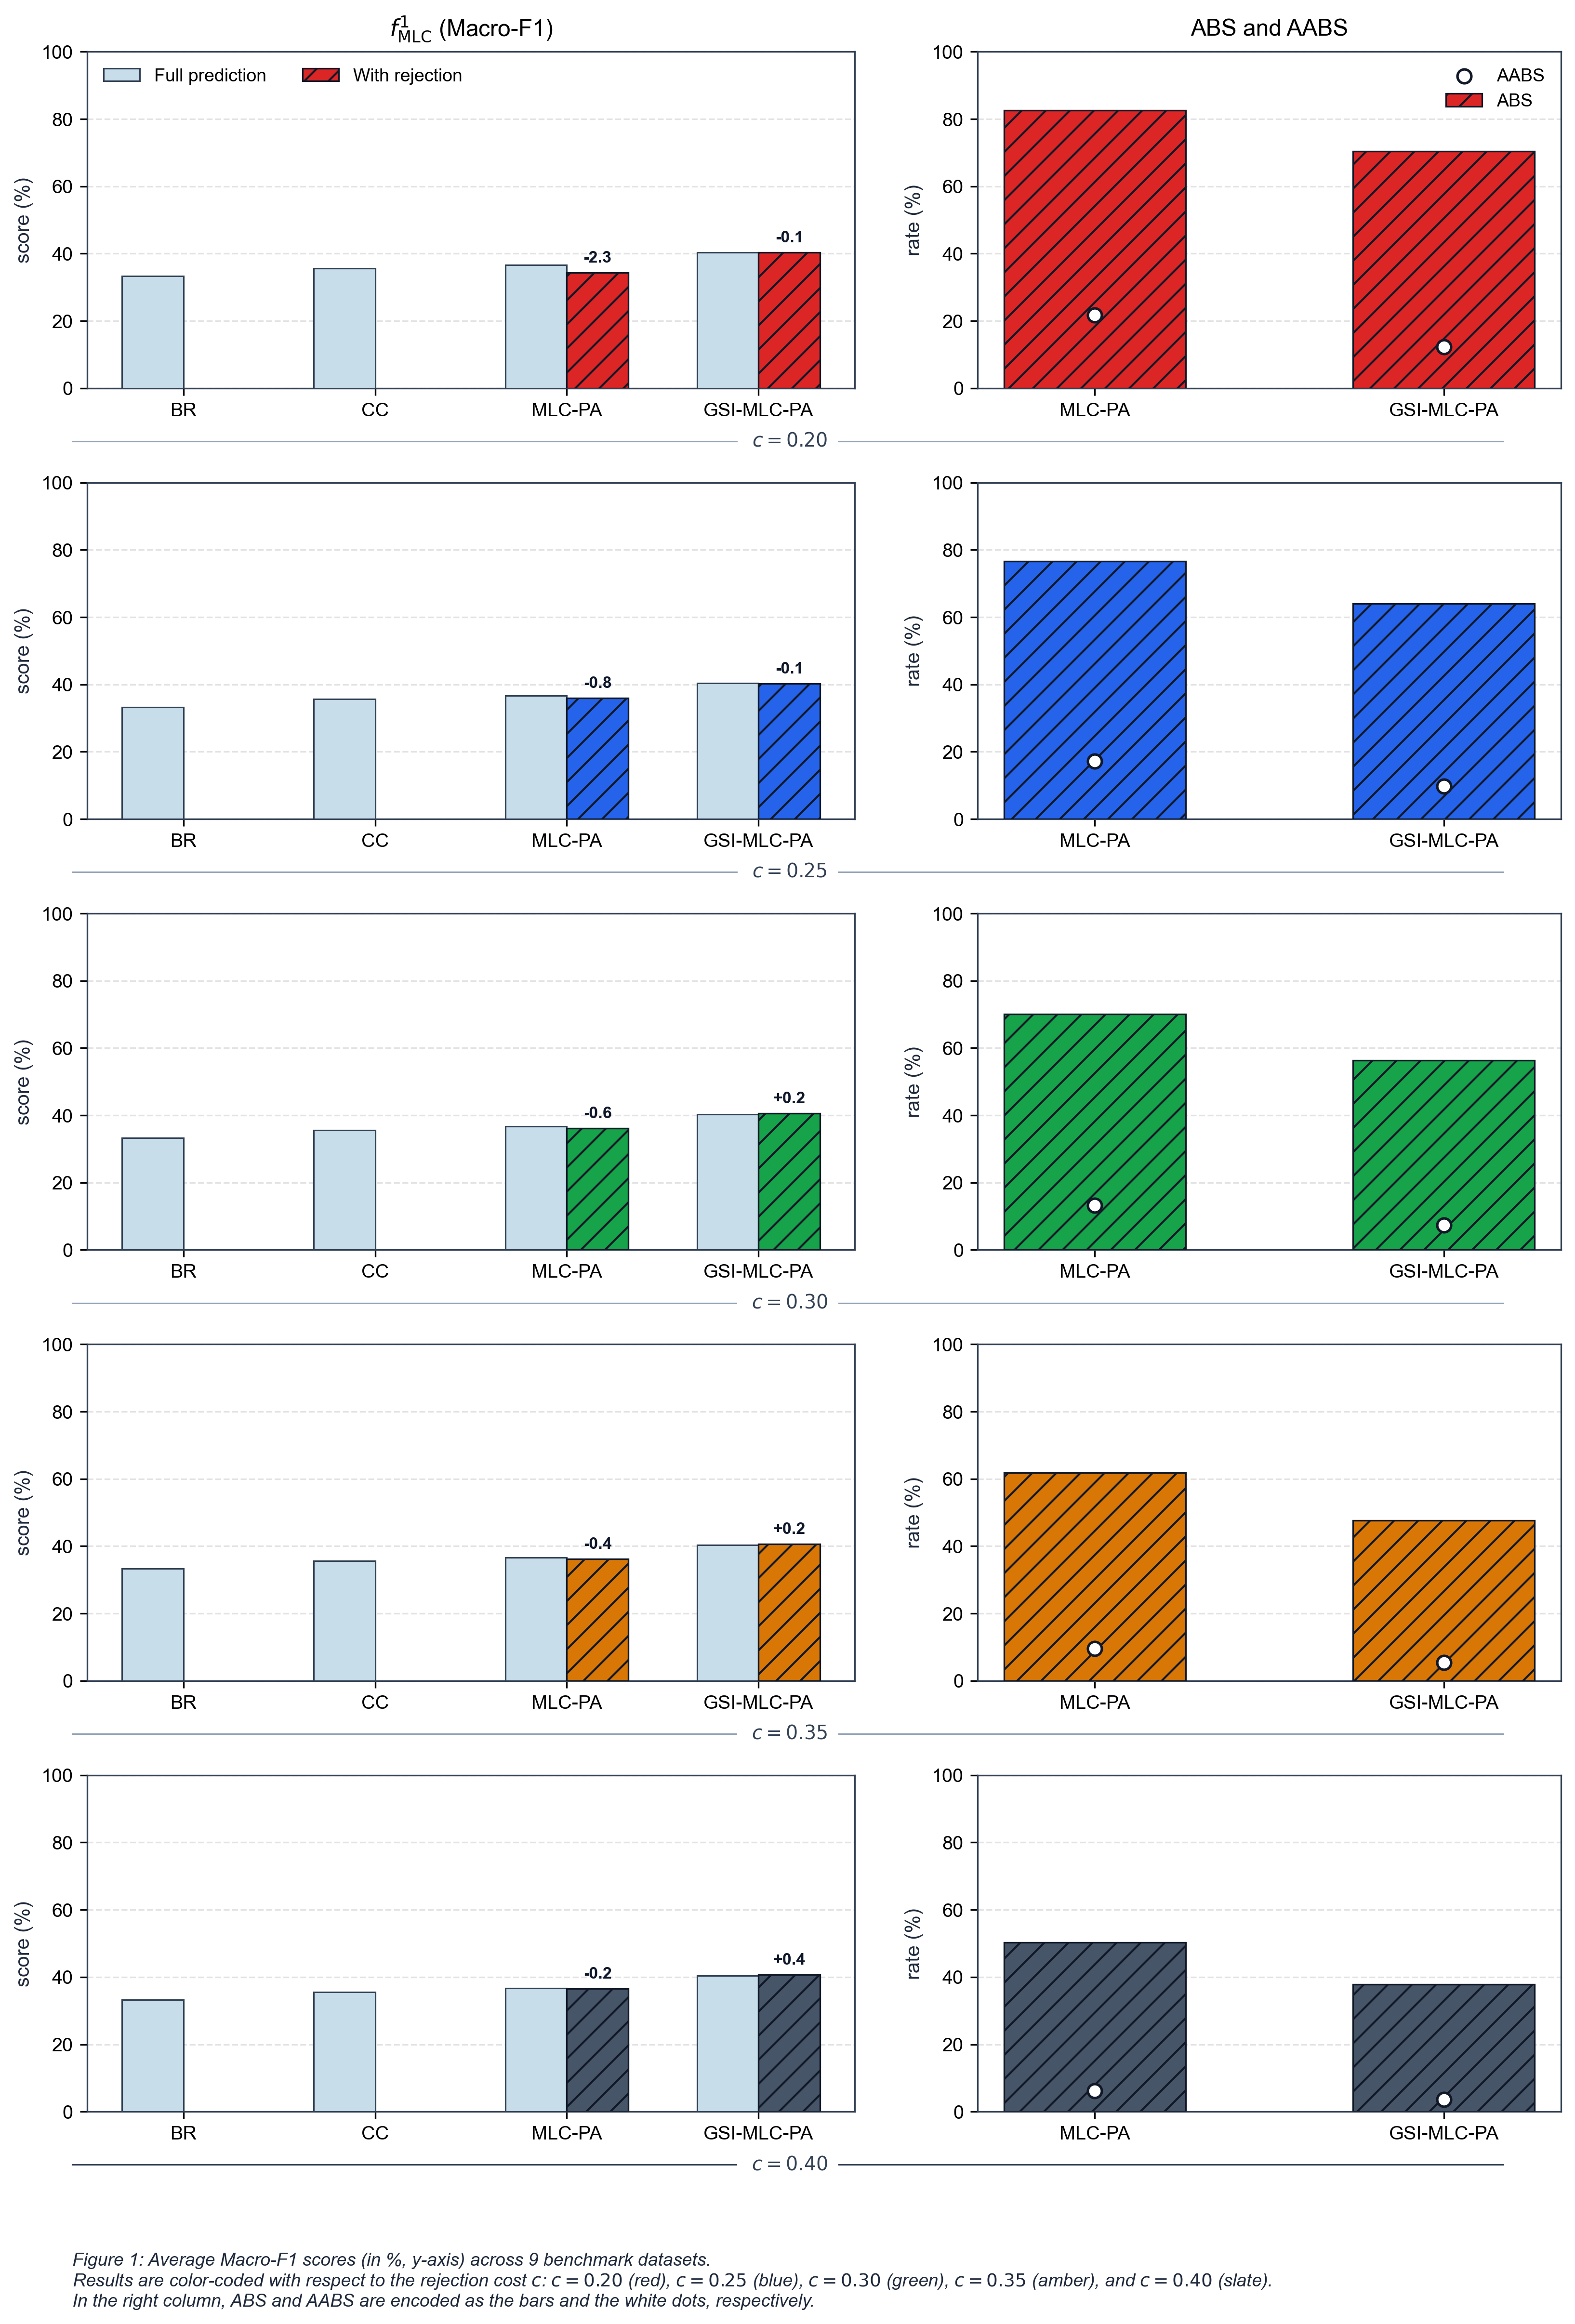
\includegraphics[width=0.92\textwidth]{figures/rejection_cost_macro_f1.png}
\caption{Đặc tính nhạy cảm chi phí và hành vi partial abstention qua các mức rejection cost $c \in \{0.20, 0.25, 0.30, 0.35, 0.40\}$ theo mô hình thực nghiệm của Nguyen và H\"ullermeier \cite{nguyen2021multilabel}. Cột trái: Điểm Macro-F1 kèm mức cải thiện delta so với complete predictions. Cột phải: Quy mô từ chối (cột gạch chéo ABS và điểm chấm tròn trắng AABS).}
\label{fig:rejection_cost_vi}
\end{figure*}

\subsubsection{Selective Classification và Human-in-the-Loop Triage}
Table \ref{tab:selective_results_vi} đánh giá partial abstention regime tại standard operating cost $c = 0.30$ dưới linear penalty.

\begin{table}[htbp]
\caption{Selective Performance và Triage Metrics ($c = 0.30$)}
\label{tab:selective_results_vi}
\centering
\begin{tabular}{lcccc}
\toprule
\textbf{Model} & \textbf{Coverage $\uparrow$} & \textbf{Gen. Loss $\downarrow$} & \textbf{ECR $\uparrow$} & \textbf{Opt. Macro-F1 $\uparrow$} \\
\midrule
MLC\_PA\_Logistic & 0.8805 & 0.0931 & 0.3841 & 0.5322 \\
MLC\_PA\_SVM & 0.8739 & 0.0950 & 0.3698 & 0.5202 \\
GSI\_MLC\_PA\_Logistic & \textbf{0.9005} & \textbf{0.0924} & 0.3474 & 0.5138 \\
GSI\_MLC\_PA\_SVM & 0.8867 & 0.0945 & 0.3413 & 0.5198 \\
GSI\_MLC\_PA\_MLP & 0.4195 & 0.1638 & \textbf{0.9041} & \textbf{0.6892} \\
\bottomrule
\end{tabular}
\end{table}

Tại cost $c = 0.30$, GSI\_MLC\_PA\_Logistic duy trì superior coverage ở mức 90.05\% với generalized loss thấp nhất (0.0924). Đáng chú ý, GSI\_MLC\_PA\_MLP chủ động abstain trên các vị trí ambiguous để thu giữ \textbf{90.41\% tổng số baseline errors} vào rejected subset ($\text{ECR} = 0.9041$), đưa human-assisted Optimistic Macro-F1 lên 0.6892. Điều này khẳng định abstention mechanism lọc chính xác high-risk predictions thay vì loại bỏ instances ngẫu nhiên, như trực quan hóa tại Fig. \ref{fig:error_capture_vi} và đường cong Risk-Coverage tại Fig. \ref{fig:risk_coverage_vi}.

\begin{figure}[htbp]
\centering
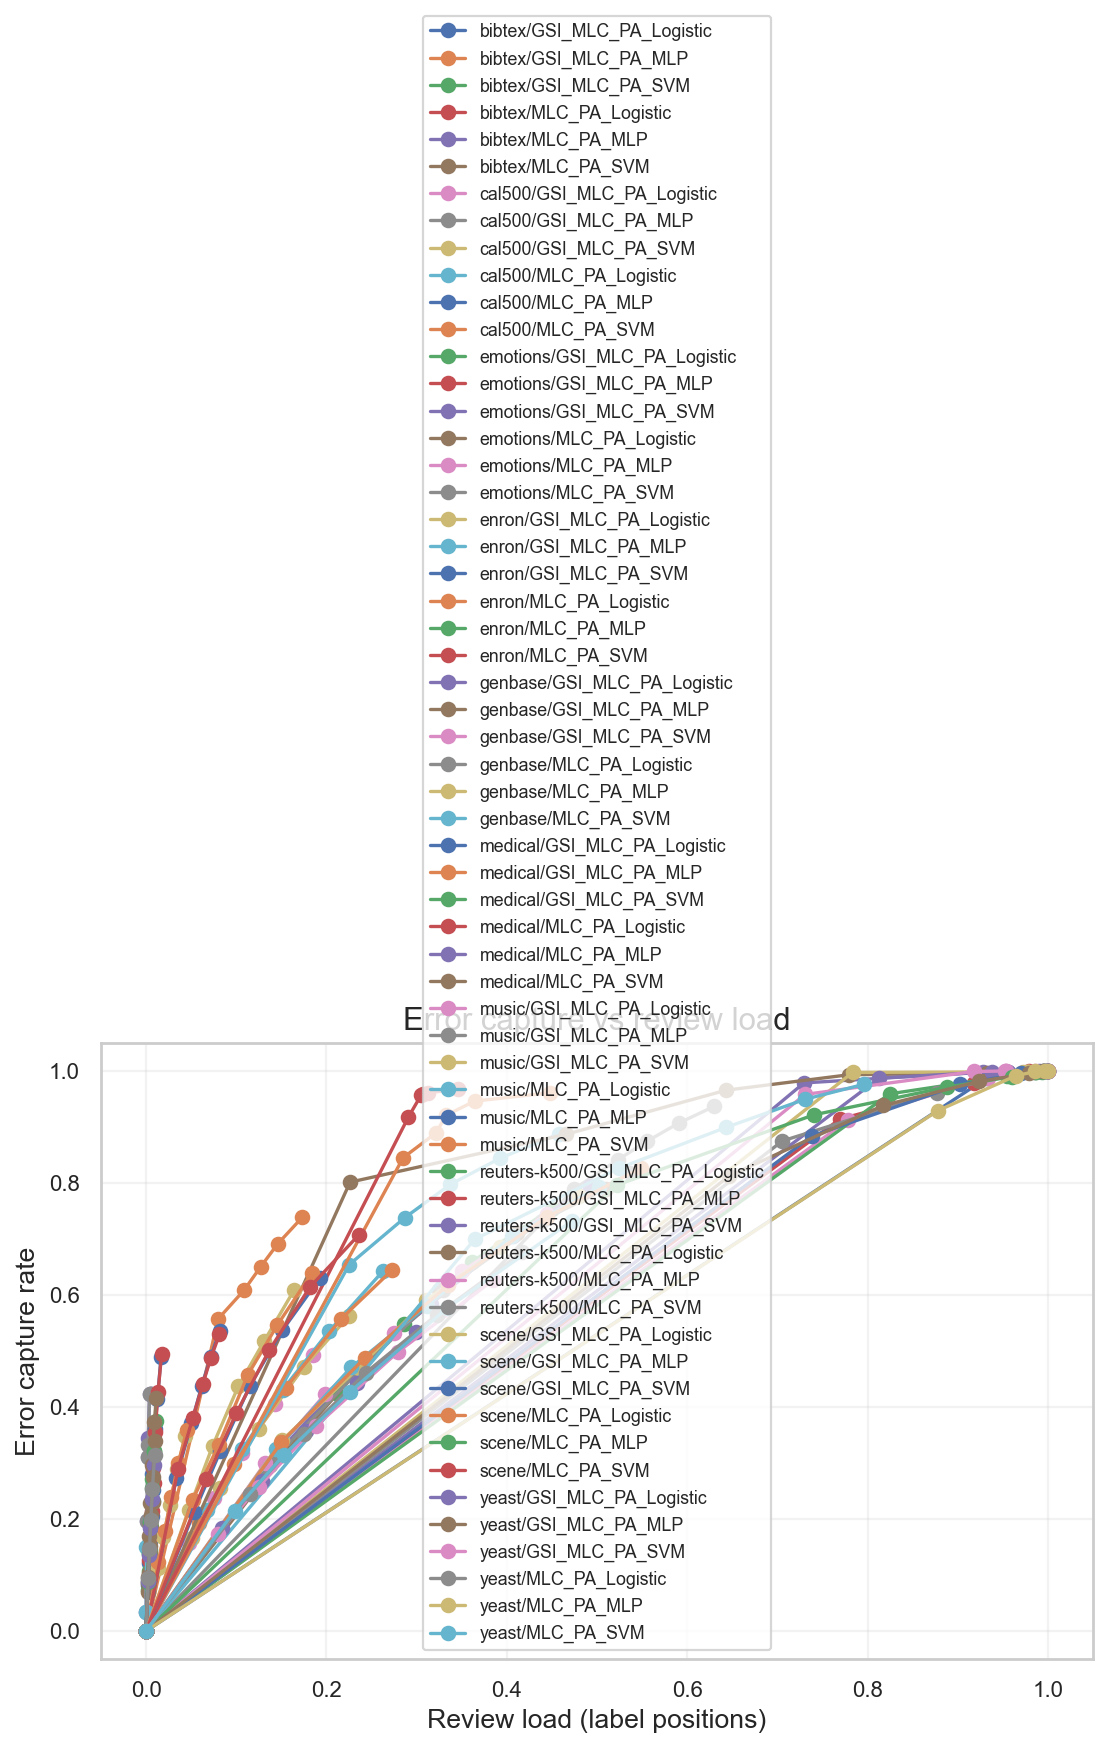
\includegraphics[width=0.92\columnwidth]{figures/error_capture_vs_review_load.png}
\caption{Error Capture Rate (ECR) so với khối lượng kiểm duyệt (AABS) trên các benchmark datasets, chứng minh partial abstention cô lập tới 90.4\% lỗi hệ thống với chi phí can thiệp của con người ở mức tối thiểu.}
\label{fig:error_capture_vi}
\end{figure}

\begin{figure}[htbp]
\centering
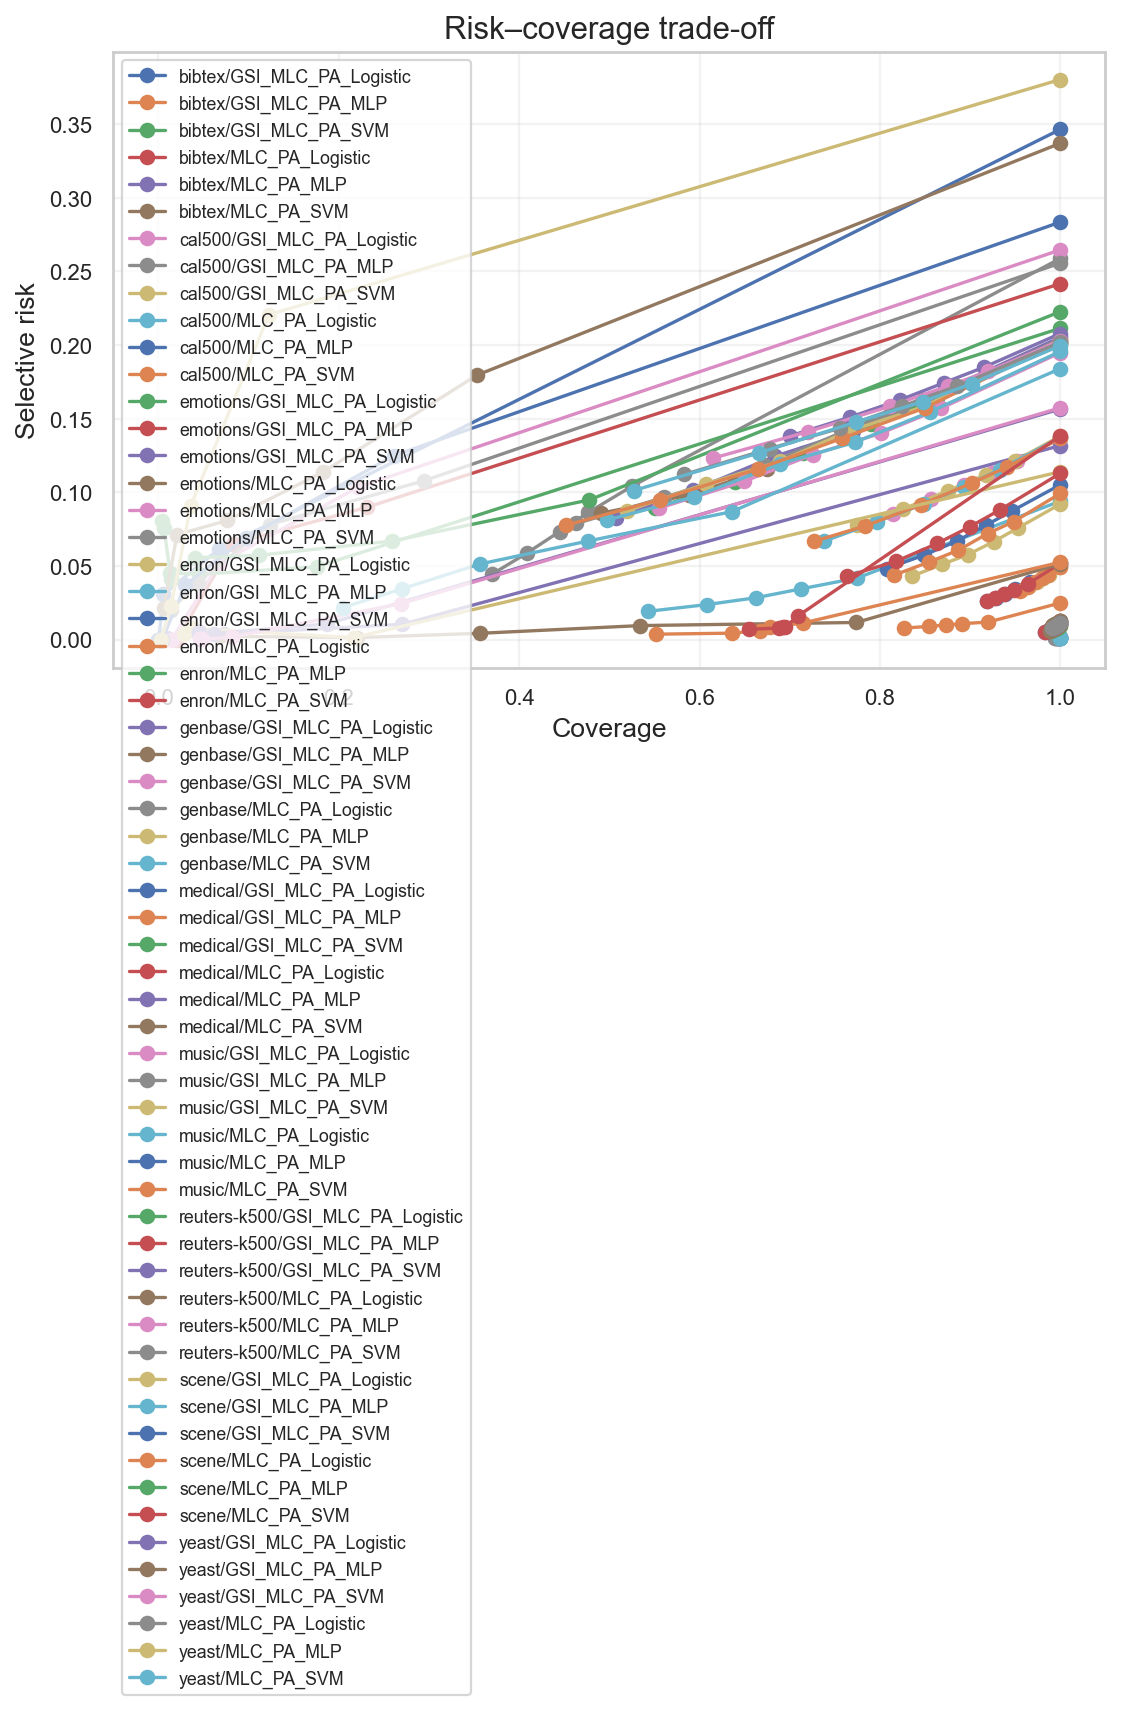
\includegraphics[width=0.92\columnwidth]{figures/risk_coverage.png}
\caption{Đặc tính đánh đổi Risk-Coverage: Selective risk giảm nhanh chóng khi mô hình thực hiện partial abstention trên các nhãn không chắc chắn, khẳng định ưu thế vượt trội của GSI-MLC-PA so với baseline.}
\label{fig:risk_coverage_vi}
\end{figure}

\subsection{Ablation Studies}

\subsubsection{IL/DL Partitioning Ablation}
Để chứng minh performance gains của GSI bắt nguồn từ adaptive partitioning chứ không đơn thuần do base learner, chúng tôi đánh giá GSI\_MLC\_PA\_Logistic trên ba controlled partition modes (trực quan hóa tại Fig. \ref{fig:il_dl_ablation_vi}):
\begin{itemize}
    \item \textbf{All-IL ($\mathcal{I} = \mathcal{L}$):} Phân rã hoàn toàn thành independent labels (tương đương BR). Macro-F1: \textbf{0.3979}.
    \item \textbf{All-DL ($\mathcal{D}_L = \mathcal{L}$):} Full linear classifier chain với correlation ordering. Macro-F1: \textbf{0.3969}.
    \item \textbf{Learned (No Correlation Reordering):} Adaptive IL/DL selection với natural label order. Macro-F1: \textbf{0.3975}.
    \item \textbf{GSI Full (Learned Partition + Correlation Order):} Macro-F1: \textbf{0.3986}.
\end{itemize}

\begin{figure}[htbp]
\centering
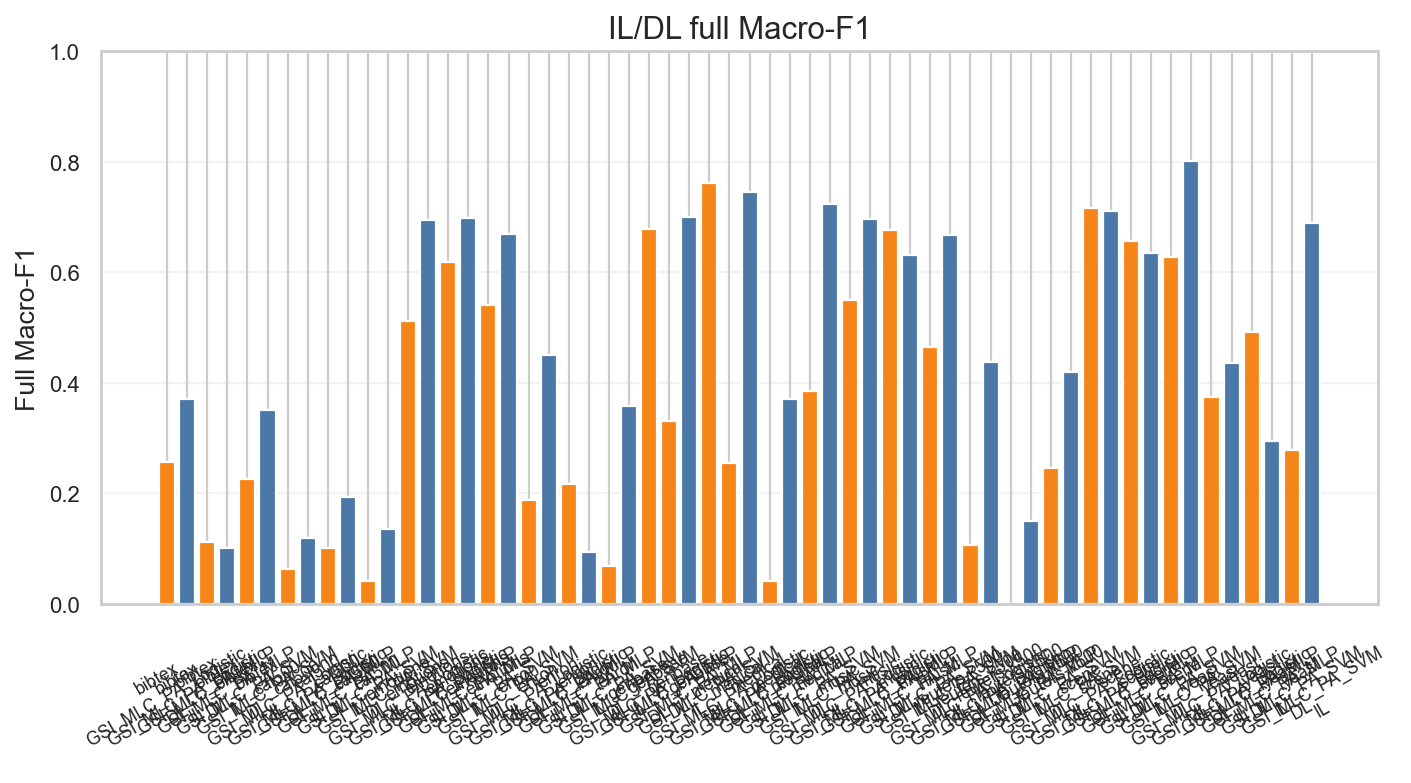
\includegraphics[width=0.95\columnwidth]{figures/il_dl_ablation.png}
\caption{Ablation phân hoạch cấu trúc IL/DL trên các benchmark datasets, xác nhận phân hoạch học được của GSI cải thiện vượt trội cả hai cấu hình cực đoan (All-IL và All-DL).}
\label{fig:il_dl_ablation_vi}
\end{figure}
Learned GSI partition vượt trội cả All-IL lower bound lẫn All-DL full chain, chứng minh việc cắt tỉa spurious dependencies giải quyết triệt để bottleneck của CC kinh điển.

\subsubsection{Selection Objective Ablation}
Chúng tôi khảo sát 6 internal validation selection objectives cho việc chọn candidate partition:
\begin{enumerate}
    \item \textit{Macro-Recall:} Macro-F1 = 0.3985, Instance-F1 = 0.5671.
    \item \textit{Full Macro-F1 (Default):} Macro-F1 = 0.3986, Instance-F1 = 0.5659.
    \item \textit{Macro-Precision:} Macro-F1 = 0.3978, Instance-F1 = 0.5636.
    \item \textit{Immediate Instance-F1:} Macro-F1 = 0.3966, Instance-F1 = 0.5652.
    \item \textit{BOP Jaccard Utility:} Macro-F1 = 0.3965, Instance-F1 = 0.5639.
    \item \textit{BOP Instance-F1 Utility:} Macro-F1 = 0.3962, Instance-F1 = 0.5647.
\end{enumerate}
Trong khi recall-oriented tuning tối ưu instance coverage, Full Macro-F1 objective mang lại sự cân bằng tối ưu giữa label-wise và instance-wise metrics.

\section{Conclusion and Future Work}
Bài báo đã đề xuất GSI-MLC-PA, một adaptive multi-label learning framework giải quyết toàn diện các hạn chế về scalability, error propagation, và uncertainty của Classifier Chains. Bằng cách phân tách label space thành independent và dependent subsets kết hợp exact và mean-field marginalization, GSI-MLC-PA đạt polynomial-time inference trong khi duy trì hoặc vượt trội predictive performance so với fully connected chains. Khi tích hợp với Bayes-optimal partial abstention layer, mô hình cô lập hiệu quả low-confidence positions, thu giữ tới 90.4\% errors phục vụ human reviewer triage.

Future work sẽ mở rộng sang active Markov Decision Process (MDP) formulations, nơi human feedback trên rejected labels được cập nhật động vào posterior distributions dọc theo chain theo thời gian thực.

\begin{thebibliography}{12}
\bibitem{zhang2018binary}
M.-L. Zhang, Y.-K. Li, X.-Y. Liu, and X. Geng, ``Binary relevance for multi-label learning: an overview,'' \emph{Frontiers of Computer Science}, vol. 12, no. 2, pp. 191--202, 2018.

\bibitem{read2011classifier}
J. Read, B. Pfahringer, G. Holmes, and E. Frank, ``Classifier chains for multi-label classification,'' \emph{Machine Learning}, vol. 85, no. 3, pp. 333--359, 2011.

\bibitem{cheng2010bayes}
W. Cheng, E. H\"ullermeier, and K. J. Dembczynski, ``Bayes optimal multilabel classification via probabilistic classifier chains,'' in \emph{Proc. 27th Int. Conf. Mach. Learn. (ICML)}, 2010, pp. 279--286.

\bibitem{dembczynski2012consistent}
K. Dembczynski, W. Cheng, and E. H\"ullermeier, ``On label dependence and loss minimization in multi-label classification,'' \emph{Machine Learning}, vol. 88, no. 1, pp. 5--45, 2012.

\bibitem{nguyen2021multilabel}
V.-L. Nguyen and E. H\"ullermeier, ``Multi-label classification with partial abstention,'' \emph{Journal of Artificial Intelligence Research}, vol. 72, pp. 1261--1316, 2021.

\bibitem{geifman2017selective}
Y. Geifman and R. El-Yaniv, ``Selective classification for deep neural networks,'' in \emph{Adv. Neural Inf. Process. Syst. (NeurIPS)}, vol. 30, 2017, pp. 4885--4894.

\bibitem{opitz2019macro}
J. Opitz and S. Burst, ``Macro f1 and macro f1? A study of evaluation metrics for multi-label classification,'' \emph{arXiv preprint arXiv:1911.03347}, 2019.

\bibitem{nam2019learning}
J. Nam, E. Loza Menc\'ia, and J. F\"urnkranz, ``Learning to search for multi-label classification,'' in \emph{Proc. 36th Int. Conf. Mach. Learn. (ICML)}, 2019, pp. 4716--4725.

\bibitem{waegeman2014bayes}
W. Waegeman, K. Dembczynski, A. Jachnik, W. Cheng, and E. H\"ullermeier, ``On the Bayes-optimality of F-measure approximators,'' \emph{Journal of Machine Learning Research}, vol. 15, no. 1, pp. 3333--3388, 2014.

\bibitem{read2012monte}
J. Read, L. Martino, and D. Luengo, ``Efficient Monte Carlo methods for multidimensional learning with classifier chains,'' \emph{Pattern Recognition}, vol. 47, no. 3, pp. 1535--1546, 2014.

\bibitem{zadrozny2002transforming}
B. Zadrozny and C. Elkan, ``Transforming classifier scores into accurate multiclass probability estimates,'' in \emph{Proc. 8th ACM SIGKDD Int. Conf. Knowl. Discov. Data Min.}, 2002, pp. 694--699.

\bibitem{scikit-learn}
F. Pedregosa \emph{et al.}, ``Scikit-learn: Machine learning in Python,'' \emph{Journal of Machine Learning Research}, vol. 12, pp. 2825--2830, 2011.
\end{thebibliography}

\end{document}
